\chapter{Preliminary experiments}

We will first perform some experiments using some simple models. These will
both serve as demonstrations that learning is feasible, and as baselines
to which we will compare results using more complex models. In addition,
we are comparing the performance of different kinds of input. We use both
tokens, character \ngrams and \ac{POS} \ngrams as inputs.


\section{Preprocessing}

The data files in the ASK corpus are in \ac{XML} format, and contain information
about tags, mistakes and corrections, paragraphs, sentences and more. These
files were transformed into several other formats during the process. First,
they were converted to plain text files, stripped of all tags or correction
labels. The text files have one sentence per line, consisting of
space-separated tokens, and an empty line separating paragraphs.

These raw text files were then sent through the UDPipe pipeline
\autocite{udpipe:2017} for tagging and dependency parsing. The UDPipe project
maintains an online REST \ac{API} containing a selection of pretrained models.
All documents were transformed by the REST \ac{API} using what was at
the time of writing the newest Norwegian bokmål (nb) model
available\footnote{\texttt{norwegian-bokmaal-ud-2.3-181115}}.

The pipeline accepts raw text files as input, where each sentence is put on a
separate line. The output from UDPipe is in the CoNLL file format, with a
single token per line. UDPipe tags the documents using the UD tagset, while
the original tags in the \ac{XML} documents are from the Oslo-Bergen tagger's own
tagset.


\section{Metrics}

The \FI score for a single class is the harmonic mean of the precision and
recall. The formula is given in equation \ref{eq:fi}, where $TP$, $FN$ and
$FP$ are the number of true positives, false negatives, and false positives,
respectively.

\begin{equation}\label{eq:fi}
  F_1 = {\frac{2\cdot TP}{2\cdot TP + FN + FP}}
\end{equation}

In a multi-class prediction setup, there are several ways to combine the
classes' individual \FI scores into a single metric. There is the micro
average \FI, which is equivalent to accuracy: The proportion of samples where
the gold labels and predicted labels are the same. Then there is the macro
average, which is the unweighted average of \FI scores for all classes. When
the distribution of classes is uneven, a macro average will give
proportionally more weight on samples from small classes, and less weight to
all samples in classes with large support. A model with a high micro \FI and
a low macro \FI indicates that it is good at classifying examples from the
most frequent classes, but performs worse on classes with low support. In
addition, the weighted \FI is a weighted average where each class is weighted
proportionally to its prevalence.

\FI scores previously reported in \ac{AES} literature include Micro \FI score
in \textcite{vajjala17}, and weighted \FI in
\textcite{vajjala18universalCEFR}. For the \ac{NLI} task, micro \FI is
reported in \textcite{malmasi15,malmasi17}.

Other, non-\FI metrics that have been reported in \ac{AES} literature include
\ac{QWK} \autocite{taghipour16, alikaniotis2016automatic}, Pearson's
correlation coefficient \autocite{vajjala17, alikaniotis2016automatic},
Spearman's rank correlation coefficient and root mean squared error
\autocite{alikaniotis2016automatic}, and mean absolute error
\autocite{vajjala17}. These are metrics that may depend on the ordinal nature
of proficiency scores, and potentially the relative differences between
different scores. For instance, a prediction of `C1' for an essay with gold
label `B1' is a more serious misclassification than a prediction of `A2/B1'
for the same sample, and this can be taken into account by some metrics.

According to \textcite{yannakoudakis2015evaluating}, \ac{QWK} is an
ill-suited metric for the task, because it depends on trait prevalence, the
scoring scale and the marginal distributions of labels and predictions.
Therefore it is problematic to compare \ac{QWK} scores between different
systems and datasets. However, since two of the cited studies are based on
a dataset from a Kaggle competition where \ac{QWK} was the official metric,
it has been reported.


\subsection{Reported metrics}

We report the macro and micro \FI for all experiments.

The metrics are reported for two different modes: The first utilizing the
full set of classes, and the second training and evaluating on the collapsed
classes.

A third option, namely to train on the full set of classes and reduce the
predictions to the collapsed set of classes, was also attempted, based on the
assumption that the more fine grained labels in the full set of classes can
provide useful supervision signals even though we evaluate on a smaller set.
However, in practice the best perforers on the collapsed labels was
empirically observed to be the models that were also trained on the collapsed
tags.


\section{Model descriptions}

Initial experiments were run using logistic regression, and \acp{MLP}, which
are simple neural networks.

\subsection{Input representations}

Input representations are shared between the linear and neural models, except
for the total number of features. The neural models may restrict the number
of features by cutting off less frequently occuring features, and this is
noted below.

\subsubsection*{Word counts}

This representation is a vector with a entry for each unique word form in the
training data, 20,766 in total. The value of each entry is the number of
times the word form occurs in the document. The neural models limits the
count vectors to the 10,000 most common tokens.

\subsubsection*{Character \ngrams}

Documents are represented by count vectors where each entry represents a
\ngram of characters. Some examples of character \ngrams are \textlangle
eg␣\textrangle, \textlangle␣i␣\textrangle\xspace or \textlangle si\textrangle. For
the linear model, all \ngrams with $n\in \{1,2,3\}$ were used, and for the
neural models the 10,000 most commonly occuring \ngrams with $n\in \{2,3,4\}$
were used.

\subsubsection*{POS \ngrams}

Documents are represented by count vectors where each entry represents a
\ngram of POS tags. Some examples of POS \ngrams are \textlangle NOUN
NOUN\textrangle, \textlangle PRON AUX PRON\textrangle or \textlangle SCONJ
ADJ\textrangle. For the linear model, all \ngrams with $n\in \{1,2,3\}$ were
used, and for the neural models the 10,000 most commonly occuring \ngrams
with $n\in \{2,3,4\}$ were used.

\subsubsection*{Mixed POS}

The Mixed POS mode was taken from \textcite{malmasi15}. Their best performing
single feature was a mix of word forms and POS tags, so that common function
words appeared in their written form, while content words were substituted
with their POS tag.

\begin{example}
\gll generasjoner kan også få   anledning til å utnytte dem
     NOUN         kan også VERB NOUN      til å VERB    dem
\glt `generations can also have the opportunity to exploit them'
\glend
\label{ex:mixed-pos}
\end{example}

Example \ref{ex:mixed-pos} shows a sentence fragment with the original series
of tokens, the sequence of mixed function words and UPOS tags it is
transformed into, as well as a translation into English.

We used the same set of stop words as \citeauthor{malmasi15}. From these
transformed sequences, we extracted \ngrams in the interval $[1,3]$. The
10,000 most commonly occuring of these were used for the neural models.


\subsection{Logistic regression}

The logistic regression model was implemented using the Python library
Scikit-Learn \autocite{scikit-learn}. The model was instantiated with the
`lgbfs' solver to minimize multinomial loss. No regularization was used, and
the optimizer was set to run for a maximum of 100 iterations.


\subsection{Multi-layer perceptron}
\label{subsec:mlp}

The MLP models were implementing in Keras \autocite{keras} and run on the
TensorFlow backend \autocite{tensorflow}. All the models the have an input
layer with 10,000 dimensions, then two fully connected layers of size 256.
The fully connected layers use \ac{ReLU} activation and dropout
regularization with a dropout rate of 50\%. At the end, there is an output
layer with softmax activation and 7 or 4 dimensions, depending on whether we
run with collapsed labels or not.

The model was trained using the Adam optimization algorithm
\autocite{kingma2014adam} to minimize the categorical cross-entropy loss
(equation \ref{eq:crossentropy}). The learning rate was set to $2\cdot
10^{-4}$.


The new \ngram features add a certain sensitivity to local order of features.
Many character \ngrams will represent entities smaller than a word, but may
indicate common spelling mistakes. \ac{POS} and Mixed POS \ngrams, on the
other hand, might be able to represent syntactic features. Spelling and
syntax should be correlated with L2 proficiency, and traditional \ac{ML}
methods that rely on manual feature engineering have included domain specific
features designed to capture spelling and syntax, as for instance in
\textcite{vajjala17}.


\section{Results}

Two different sets of output labels are used in the experiments: The original
seven CEFR labels, and a collapsed set where the intermediate classes, such
as ``A2/B1'', are rounded up to the nearest canonical class, i.e. the CEFR
label after the slash. This results in only four different labels: ``A2'',
``B1'', ``B2'' and ``C1''.

As a simple baseline, we consider the majority class classifier. The majority
class in the training set is ``B1'', whether we consider the full class set
or the collapsed set. A majority classifier gets an accuracy of 18.7\% on the
test set using non-collapsed labels. With the collapsed labels, the accuracy
on the test set is 34.1\%. The macro \FI scores are much lower, as the
majority class classifier predicts no samples for any other classes.

Moving to a linear model, a logistic regression classifier using only
bag-of-word features achieves an accuracy of 28.5\% on the dev set without
collapsed labels and 58.5\% with collapsed labels. However, the linear model
that performs the best is the one using character \ngrams.

\begin{table}
  \centering
  \begin{tabular}{lrrrr}
    \toprule
             & \multicolumn{2}{c}{All labels} & \multicolumn{2}{c}{Collapsed labels} \\
    \cmidrule(lr){2-3}
    \cmidrule(lr){4-5}
    Model      & Macro \FI       & Micro \FI       & Macro \FI       & Micro \FI      \\
    \midrule
    Majority   &         $0.040$  &         $0.163$  &         $0.127$  &         $0.341$ \\
    \midrule
    LogReg BOW &         $0.199$  &         $0.317$  &         $0.384$  &         $0.626$ \\
    LogReg Char&         $0.221$  &         $0.317$  &         $0.399$  &         $0.602$ \\
    LogReg POS &         $0.188$  &         $0.276$  &         $0.344$  &         $0.585$ \\
    LogReg Mix &         $0.213$  &         $0.341$  &         $0.342$  &         $0.585$ \\
    \midrule
    % $BEGIN autotable baseline-accuracies
    % $META models-per-row=2 columns-per-model=macrof1,microf1
    % $ROW MLP BOW:    mlp_word-03-01_11-53-35    mlp_word-03-01_11-55-36
    % $ROW MLP Char:   mlp_char-03-01_11-57-23    mlp_char-03-01_11-59-00
    % $ROW MLP POS:    mlp_pos-03-01_12-00-44     mlp_pos-03-01_12-02-31
    % $ROW MLP Mix:    mlp_mixed-02-20_14-45-16   mlp_mixed-02-22_13-43-37
    % $END autotable
    MLP BOW & $0.209$ & $0.366$ & $0.392$ & $0.642$ \\
    MLP Char & $\mathbf{0.281}$ & $\mathbf{0.472}$ & $0.423$ & $0.659$ \\
    MLP POS & $0.245$ & $0.366$ & $\mathbf{0.439}$ & $\mathbf{0.691}$ \\
    MLP Mix & $0.239$ & $0.398$ & $0.384$ & $0.667$ \\
    \bottomrule
  \end{tabular}
  \caption{\FI scores of different classifiers}
  \label{tab:baseline-accuracies}
\end{table}

All results are seen in table \ref{tab:baseline-accuracies}.
The part of speech \ngrams performed best overall, having the highest \FI score
for the full label set, both for macro and micro average. On the collapsed set
of labels, the part of speech \ngrams had the highest macro \FI score, but were
beat in micro \FI by the character \ngrams.

Confusion matrices from MLP Mix:

\begin{figure}
  \centering
  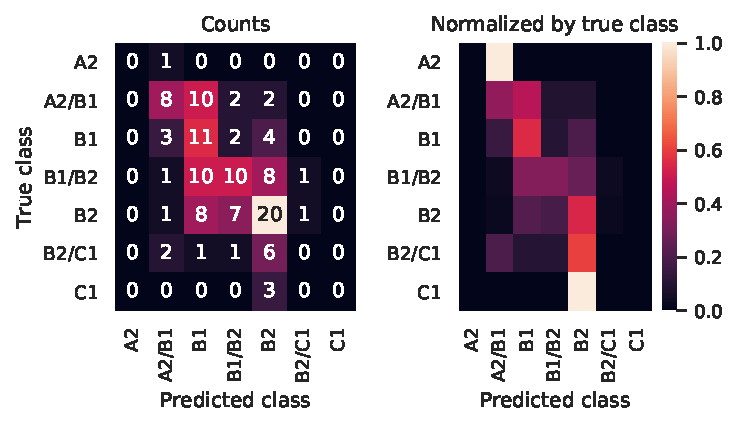
\includegraphics{mlp-mixed-conf}
  \caption{Confusion matrix for MLP Mix}
  \label{fig:mlp-mixed-conf}
\end{figure}

\begin{figure}
  \centering
  \includegraphics{mlp-mixed-conf-round}
  \caption{Confusion matrix for MLP Mix on collapsed labels}
  \label{fig:mlp-mixed-conf-round}
\end{figure}
